\documentclass[12pt,letterpaper,fleqn]{hmcpset}
\usepackage[margin=1in]{geometry}
\usepackage{graphicx}
\usepackage{amsmath,amssymb}
\usepackage{enumerate}
\usepackage{hyperref}
\usepackage{parskip}

% Theorems
\usepackage{amsthm}
\renewcommand\qedsymbol{$\blacksquare$}
\makeatletter
\@ifclassloaded{article}{
    \newtheorem{definition}{Definition}[section]
    \newtheorem{example}{Example}[section]
    \newtheorem{theorem}{Theorem}[section]
    \newtheorem{corollary}{Corollary}[theorem]
    \newtheorem{lemma}{Lemma}[theorem]
}{
}
\makeatother

% Random Stuff
\setlength\unitlength{1mm}

\newcommand{\insertfig}[3]{
\begin{figure}[htbp]\begin{center}\begin{picture}(120,90)
\put(0,-5){\includegraphics[width=12cm,height=9cm,clip=]{#1.eps}}\end{picture}\end{center}
\caption{#2}\label{#3}\end{figure}}

\newcommand{\insertxfig}[4]{
\begin{figure}[htbp]
\begin{center}
\leavevmode \centerline{\resizebox{#4\textwidth}{!}{\input
#1.pstex_t}}
\caption{#2} \label{#3}
\end{center}
\end{figure}}

\long\def\comment#1{}

\newcommand\norm[1]{\left\lVert#1\right\rVert}
\DeclareMathOperator*{\argmin}{arg\,min}
\DeclareMathOperator*{\argmax}{arg\,max}

% bb font symbols
\newfont{\bbb}{msbm10 scaled 700}
\newcommand{\CCC}{\mbox{\bbb C}}

\newfont{\bbf}{msbm10 scaled 1100}
\newcommand{\CC}{\mbox{\bbf C}}
\newcommand{\PP}{\mbox{\bbf P}}
\newcommand{\RR}{\mbox{\bbf R}}
\newcommand{\QQ}{\mbox{\bbf Q}}
\newcommand{\ZZ}{\mbox{\bbf Z}}
\renewcommand{\SS}{\mbox{\bbf S}}
\newcommand{\FF}{\mbox{\bbf F}}
\newcommand{\GG}{\mbox{\bbf G}}
\newcommand{\EE}{\mbox{\bbf E}}
\newcommand{\NN}{\mbox{\bbf N}}
\newcommand{\KK}{\mbox{\bbf K}}
\newcommand{\KL}{\mbox{\bbf KL}}

% Vectors
\renewcommand{\aa}{{\bf a}}
\newcommand{\bb}{{\bf b}}
\newcommand{\cc}{{\bf c}}
\newcommand{\dd}{{\bf d}}
\newcommand{\ee}{{\bf e}}
\newcommand{\ff}{{\bf f}}
\renewcommand{\gg}{{\bf g}}
\newcommand{\hh}{{\bf h}}
\newcommand{\ii}{{\bf i}}
\newcommand{\jj}{{\bf j}}
\newcommand{\kk}{{\bf k}}
\renewcommand{\ll}{{\bf l}}
\newcommand{\mm}{{\bf m}}
\newcommand{\nn}{{\bf n}}
\newcommand{\oo}{{\bf o}}
\newcommand{\pp}{{\bf p}}
\newcommand{\qq}{{\bf q}}
\newcommand{\rr}{{\bf r}}
\renewcommand{\ss}{{\bf s}}
\renewcommand{\tt}{{\bf t}}
\newcommand{\uu}{{\bf u}}
\newcommand{\ww}{{\bf w}}
\newcommand{\vv}{{\bf v}}
\newcommand{\xx}{{\bf x}}
\newcommand{\yy}{{\bf y}}
\newcommand{\zz}{{\bf z}}
\newcommand{\0}{{\bf 0}}
\newcommand{\1}{{\bf 1}}

% Matrices
\newcommand{\Ab}{{\bf A}}
\newcommand{\Bb}{{\bf B}}
\newcommand{\Cb}{{\bf C}}
\newcommand{\Db}{{\bf D}}
\newcommand{\Eb}{{\bf E}}
\newcommand{\Fb}{{\bf F}}
\newcommand{\Gb}{{\bf G}}
\newcommand{\Hb}{{\bf H}}
\newcommand{\Ib}{{\bf I}}
\newcommand{\Jb}{{\bf J}}
\newcommand{\Kb}{{\bf K}}
\newcommand{\Lb}{{\bf L}}
\newcommand{\Mb}{{\bf M}}
\newcommand{\Nb}{{\bf N}}
\newcommand{\Ob}{{\bf O}}
\newcommand{\Pb}{{\bf P}}
\newcommand{\Qb}{{\bf Q}}
\newcommand{\Rb}{{\bf R}}
\newcommand{\Sb}{{\bf S}}
\newcommand{\Tb}{{\bf T}}
\newcommand{\Ub}{{\bf U}}
\newcommand{\Wb}{{\bf W}}
\newcommand{\Vb}{{\bf V}}
\newcommand{\Xb}{{\bf X}}
\newcommand{\Yb}{{\bf Y}}
\newcommand{\Zb}{{\bf Z}}

% Calligraphic
\newcommand{\Ac}{{\cal A}}
\newcommand{\Bc}{{\cal B}}
\newcommand{\Cc}{{\cal C}}
\newcommand{\Dc}{{\cal D}}
\newcommand{\Ec}{{\cal E}}
\newcommand{\Fc}{{\cal F}}
\newcommand{\Gc}{{\cal G}}
\newcommand{\Hc}{{\cal H}}
\newcommand{\Ic}{{\cal I}}
\newcommand{\Jc}{{\cal J}}
\newcommand{\Kc}{{\cal K}}
\newcommand{\Lc}{{\cal L}}
\newcommand{\Mc}{{\cal M}}
\newcommand{\Nc}{{\cal N}}
\newcommand{\Oc}{{\cal O}}
\newcommand{\Pc}{{\cal P}}
\newcommand{\Qc}{{\cal Q}}
\newcommand{\Rc}{{\cal R}}
\newcommand{\Sc}{{\cal S}}
\newcommand{\Tc}{{\cal T}}
\newcommand{\Uc}{{\cal U}}
\newcommand{\Wc}{{\cal W}}
\newcommand{\Vc}{{\cal V}}
\newcommand{\Xc}{{\cal X}}
\newcommand{\Yc}{{\cal Y}}
\newcommand{\Zc}{{\cal Z}}

% Bold greek letters
\newcommand{\alphab}{\hbox{\boldmath$\alpha$}}
\newcommand{\betab}{\hbox{\boldmath$\beta$}}
\newcommand{\gammab}{\hbox{\boldmath$\gamma$}}
\newcommand{\deltab}{\hbox{\boldmath$\delta$}}
\newcommand{\etab}{\hbox{\boldmath$\eta$}}
\newcommand{\lambdab}{\hbox{\boldmath$\lambda$}}
\newcommand{\epsilonb}{\hbox{\boldmath$\epsilon$}}
\newcommand{\nub}{\hbox{\boldmath$\nu$}}
\newcommand{\mub}{\hbox{\boldmath$\mu$}}
\newcommand{\zetab}{\hbox{\boldmath$\zeta$}}
\newcommand{\phib}{\hbox{\boldmath$\phi$}}
\newcommand{\psib}{\hbox{\boldmath$\psi$}}
\newcommand{\thetab}{\hbox{\boldmath$\theta$}}
\newcommand{\taub}{\hbox{\boldmath$\tau$}}
\newcommand{\omegab}{\hbox{\boldmath$\omega$}}
\newcommand{\xib}{\hbox{\boldmath$\xi$}}
\newcommand{\sigmab}{\hbox{\boldmath$\sigma$}}
\newcommand{\pib}{\hbox{\boldmath$\pi$}}
\newcommand{\rhob}{\hbox{\boldmath$\rho$}}

\newcommand{\Gammab}{\hbox{\boldmath$\Gamma$}}
\newcommand{\Lambdab}{\hbox{\boldmath$\Lambda$}}
\newcommand{\Deltab}{\hbox{\boldmath$\Delta$}}
\newcommand{\Sigmab}{\hbox{\boldmath$\Sigma$}}
\newcommand{\Phib}{\hbox{\boldmath$\Phi$}}
\newcommand{\Pib}{\hbox{\boldmath$\Pi$}}
\newcommand{\Psib}{\hbox{\boldmath$\Psi$}}
\newcommand{\Thetab}{\hbox{\boldmath$\Theta$}}
\newcommand{\Omegab}{\hbox{\boldmath$\Omega$}}
\newcommand{\Xib}{\hbox{\boldmath$\Xi$}}

% mixed symbols
\newcommand{\sinc}{{\hbox{sinc}}}
\newcommand{\diag}{{\hbox{diag}}}
\renewcommand{\det}{{\hbox{det}}}
\newcommand{\trace}{{\hbox{tr}}}
\newcommand{\tr}{\trace}
\newcommand{\sign}{{\hbox{sign}}}
\renewcommand{\arg}{{\hbox{arg}}}
\newcommand{\var}{{\hbox{var}}}
\newcommand{\cov}{{\hbox{cov}}}
\renewcommand{\Re}{{\rm Re}}
\renewcommand{\Im}{{\rm Im}}
\newcommand{\eqdef}{\stackrel{\Delta}{=}}
\newcommand{\defines}{{\,\,\stackrel{\scriptscriptstyle \bigtriangleup}{=}\,\,}}
\newcommand{\<}{\left\langle}
\renewcommand{\>}{\right\rangle}
\newcommand{\Psf}{{\sf P}}
\newcommand{\T}{\top}
\newcommand{\m}[1]{\begin{bmatrix} #1 \end{bmatrix}}


% info for header block in upper right hand corner
\name{}
\class{Math189R SP19}
\assignment{Homework 8}
\duedate{Thursday, Apr 15, 2019}

\begin{document}

Feel free to work with other students, but make sure you write up the homework
and code on your own (no copying homework \textit{or} code; no pair programming).
Feel free to ask students or instructors for help debugging code or whatever else,
though.
\newline
\newline
The starter files for problem 1 and extra credit can be found under the Resource tab on course website. Please print out all the graphs generated by your own code and submit them together with the written part, and make sure you upload the code to your Github repository.



\begin{problem}[1]
\textbf{(K-means)} In this problem, we will implement the k-means algorithm and separate 5,000 2D data points into different number of clusters.
\newline
\par Let $X = {x_1, x_2 \ldots, x_m} $ be the data points, and let $k$ be the number of clusters. The k-means algorithm is summarized as following:
\begin{enumerate}[1.]
\item Randomly initialize $k$ cluster centers, $\mu_1, \mu_2 \ldots \mu_k$, in the feature space.
\item Calculate the distance between each data points and the cluster centers.
\item Assign each data point to the cluster center $c$ whose distance between this data point is the minimum of all the cluster centers, namely, \[
c_i = \argmin_j ||x_i - \mu_j||^2
\]
\item Update each cluster center to be\[
\mu_j = \frac{\sum_{i=1}^{m}1\{c_i = j\}x_i}{\sum_{i = 1}^{m}1\{c_i = j\}}
\]
\item Repeat step 2 - 4 until convergence or exhausted.
\end{enumerate}
\par 
The objective (cost) function is defined as \[
J(c, \mu) = \sum_{i = 1}^{m}||x_i - \mu_{c_i}||^2
\]

\par In this assignment, you will first implement the k-means cost function and the algorithm. Then, for $k = 1, 2 \ldots, 20$, find the number of clusters with the optimal cost and produce a plot of the relationship between the cost and the number of clusters. Then, visualize the data points and the cluster centers on the optimal number of clusters.
\newline 
\par Notice that the k-means algorithm might yield different results based on the randomness of the initialization of cluster centers.
\end{problem}
\begin{solution}
\begin{center}
	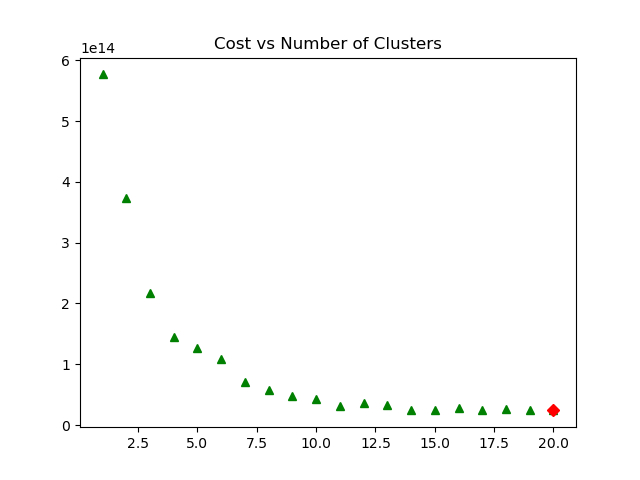
\includegraphics[scale=0.9]{kmeans_1.png}
	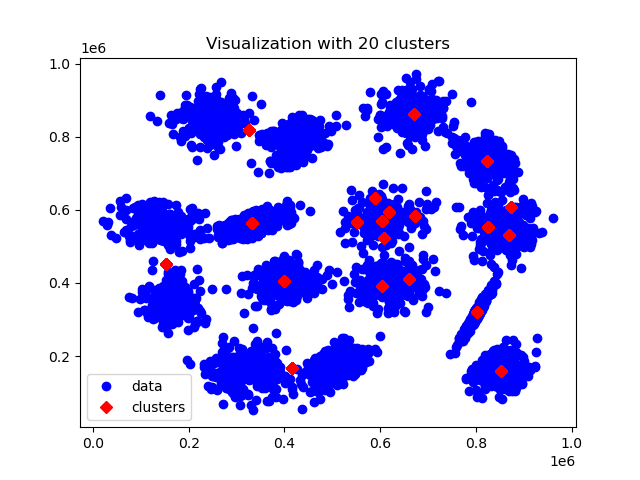
\includegraphics[scale=0.9]{kmeans_2.png}
\end{center}
\end{solution}
\newpage




\begin{problem}[Extra Credit]
\textbf{(Non-Negative Matrix Factorization)} 
In this problem, we will use the reuters dataset in nltk library. Please run nltk.download() in python shell to download the dataset. In the starter code, we have already parsed the data for you. 
\newline
\newline
Choosing an appropriate
objective function and algorithm from Lee and Seung 2001\footnote{\url{https://papers.nips.cc/paper/1861-algorithms-for-non-negative-matrix-factorization.pdf}}
implement Non-Negative Matrix Factorization for topic modelling (choose an appropriate number
of topics/latent features) and assert that the convergence properties proved in the paper hold. 
Display the 20 most relevant words for each of the topics you discover.
\end{problem}
\begin{solution}
\vfill
\end{solution}
\newpage

\begin{problem}[Extra Credit]
\textbf{(Linear Regression)} Consider the Bayesian Linear Regression model with
the following generative process:
\begin{enumerate}[(1)]
    \item Draw $\ww \sim \Nc(\0, \mathbf{V}_0)$
    \item Draw $\yy_i \sim \Nc(\ww^\T\xx_i, \sigma^2)$ for $i=1,2,\dots,n$ where $\sigma^2$
        is known.
\end{enumerate}
Express this model as a directed graphical model using Plate notation. Is $\yy_i$
independent of $\ww$? Is $\yy_i$ independent of $\ww$ \textit{given} $\Dc = \{\xx_i\}$? Support
these claims.
\end{problem}
\begin{solution}
\vfill
\end{solution}
\newpage






\end{document}
